\documentclass[11pt,a4paper]{jarticle}
\usepackage[dvipdfmx]{graphicx}
\usepackage{url}

\renewcommand{\baselinestretch}{1.05} 
\marginparwidth=0cm
\topmargin=-1cm
\headheight=0.3cm
\headsep=0.7cm
\oddsidemargin=0cm
\evensidemargin=0cm
%\textwidth=43zw
\textwidth=15.92cm
%\textheight=43.3\baselineskip
\baselineskip = 0.5744cm
\textheight=43\baselineskip

\itemsep=0.05\baselineskip
\parsep=0pt
\topsep=0.01\baselineskip
\partopsep=0pt
\listparindent=0zw

%% header and footer
\usepackage{fancyhdr}
\pagestyle{fancy}
\lhead{2016年度 春学期授業}
\chead{インタラクティブ・アート実習}
\rhead{担当教員: 松下 光範}
\cfoot{\thepage}
\renewcommand{\headrulewidth}{0pt}
\renewcommand{\footrulewidth}{0pt}

\usepackage{ascmac}
\usepackage{listings,jlisting}
\usepackage{color}
\definecolor{OliveGreen}{cmyk}{0.64,0,0.95,0.40}
\definecolor{colFunc}{rgb}{1,0.07,0.54}
\definecolor{CadetBlue}{cmyk}{0.62,0.57,0.23,0}
\definecolor{Brown}{cmyk}{0,0.81,1,0.60}
\definecolor{colID}{rgb}{0.63,0.44,0}
\definecolor{rulesepcolor}{gray}{0.666}
\lstset{
  language=Java,%プログラミング言語によって変える。
  basicstyle={\ttfamily\small},
  keywordstyle={\color{OliveGreen}},
  %[2][3]はプログラミング言語によってあったり、なかったり
  keywordstyle={[2]\color{colFunc}},
  keywordstyle={[3]\color{CadetBlue}},%
  commentstyle={\color{Brown}},
  %identifierstyle={\color{colID}},
  stringstyle=\color{blue},
  tabsize=2,
  %frame=trBL,
  %numbers=left,
  numberstyle={\ttfamily\small},
  breaklines=true,%折り返し
  %backgroundcolor={\color[gray]{.95}},
  framexleftmargin=0mm,
  frame=single,
  rulesepcolor=\color{rulesepcolor},
  captionpos=b
}


%%%%%%%%%%%%%%%%%%%%%%%%%%%%%%%%%%%%%%%%%%%%%%%%%%%%%%%%%%%%%%%%
\begin{document}

% title
\section*{\LARGE{第7講 応用編: 赤外線センサとモーターを連携させる}}
\section{本実習の目標}
\begin{itemize}
 \item モーターの回転速度を制御する。
 \item 測定した距離に応じてモーターの回転数を制御する。
\end{itemize}

%%%%%%%%%%%%%%%%%%%%%%%%%%%%%%%%%%%%%%%%%%%%%%%%%%%%%%%%%%%%%%%%

\section{モーターの回転速度を制御する}
モーターを制御する回路にはいくつか種類がありますが、今回は配線が簡単な電界効果トランジスタ (FET: Field effect transistor) を使用した回路を用います。
モーターを回転させるには、比較的大きな電流が必要なため、Arduino の出力だけでは、モーターを回転させ続けるパワーが足りません。
そのため、外部電源からモーターに電力を供給し、Arduino や Processing で制御するために必要となるのが FET です。
FET を用いることで、モーターに流す電流を制御し、モーターの回転数を変化させることができます (電流が多く流れると早く回る)。また、FETは「金属酸化膜型 (MOSFET) 」「接合系 (JFET) 」「金属半導体系 (MSEFET) 」等がありますが、本実習ではMOSFET (Metal-oxide-semiconductor field-effect transistor) を用います。

\subsection*{用いる部品}
今回は簡単にするためにに外部電源を使わずにやってみます。
各部品が手元にあるか確認してください。
\begin{figure}[h!]
 \begin{minipage}{0.32\columnwidth}
  \centering
  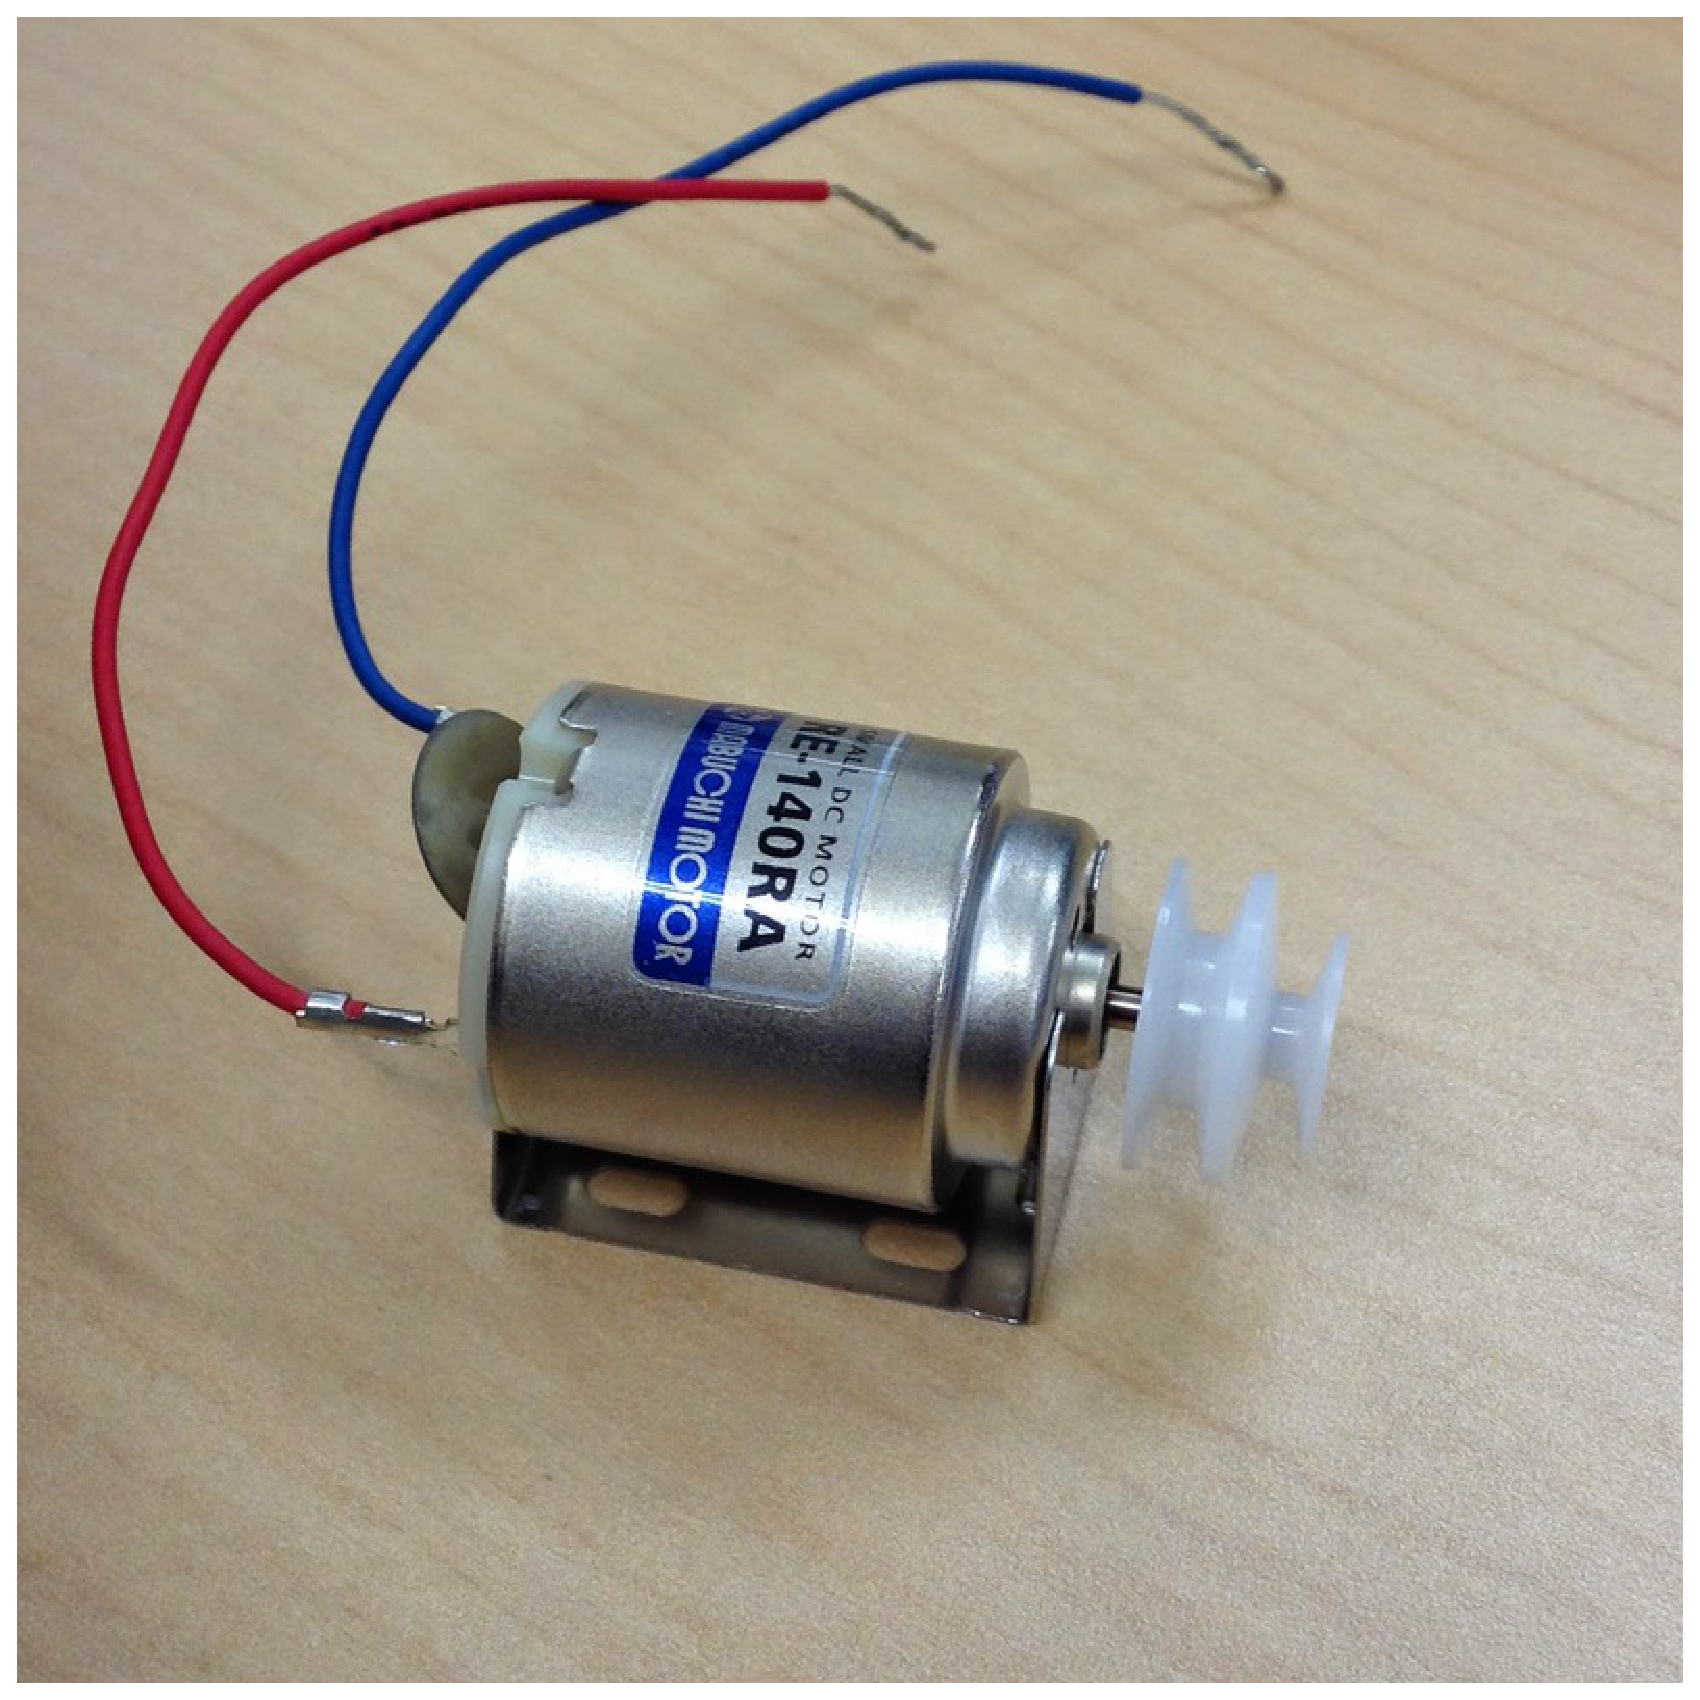
\includegraphics[width=\columnwidth]{img/motor.eps}
  \begin{center}
   \textbf{モーター(RE-140RA)}
  \end{center}
 \end{minipage}
 \begin{minipage}{0.32\columnwidth}
  \centering
  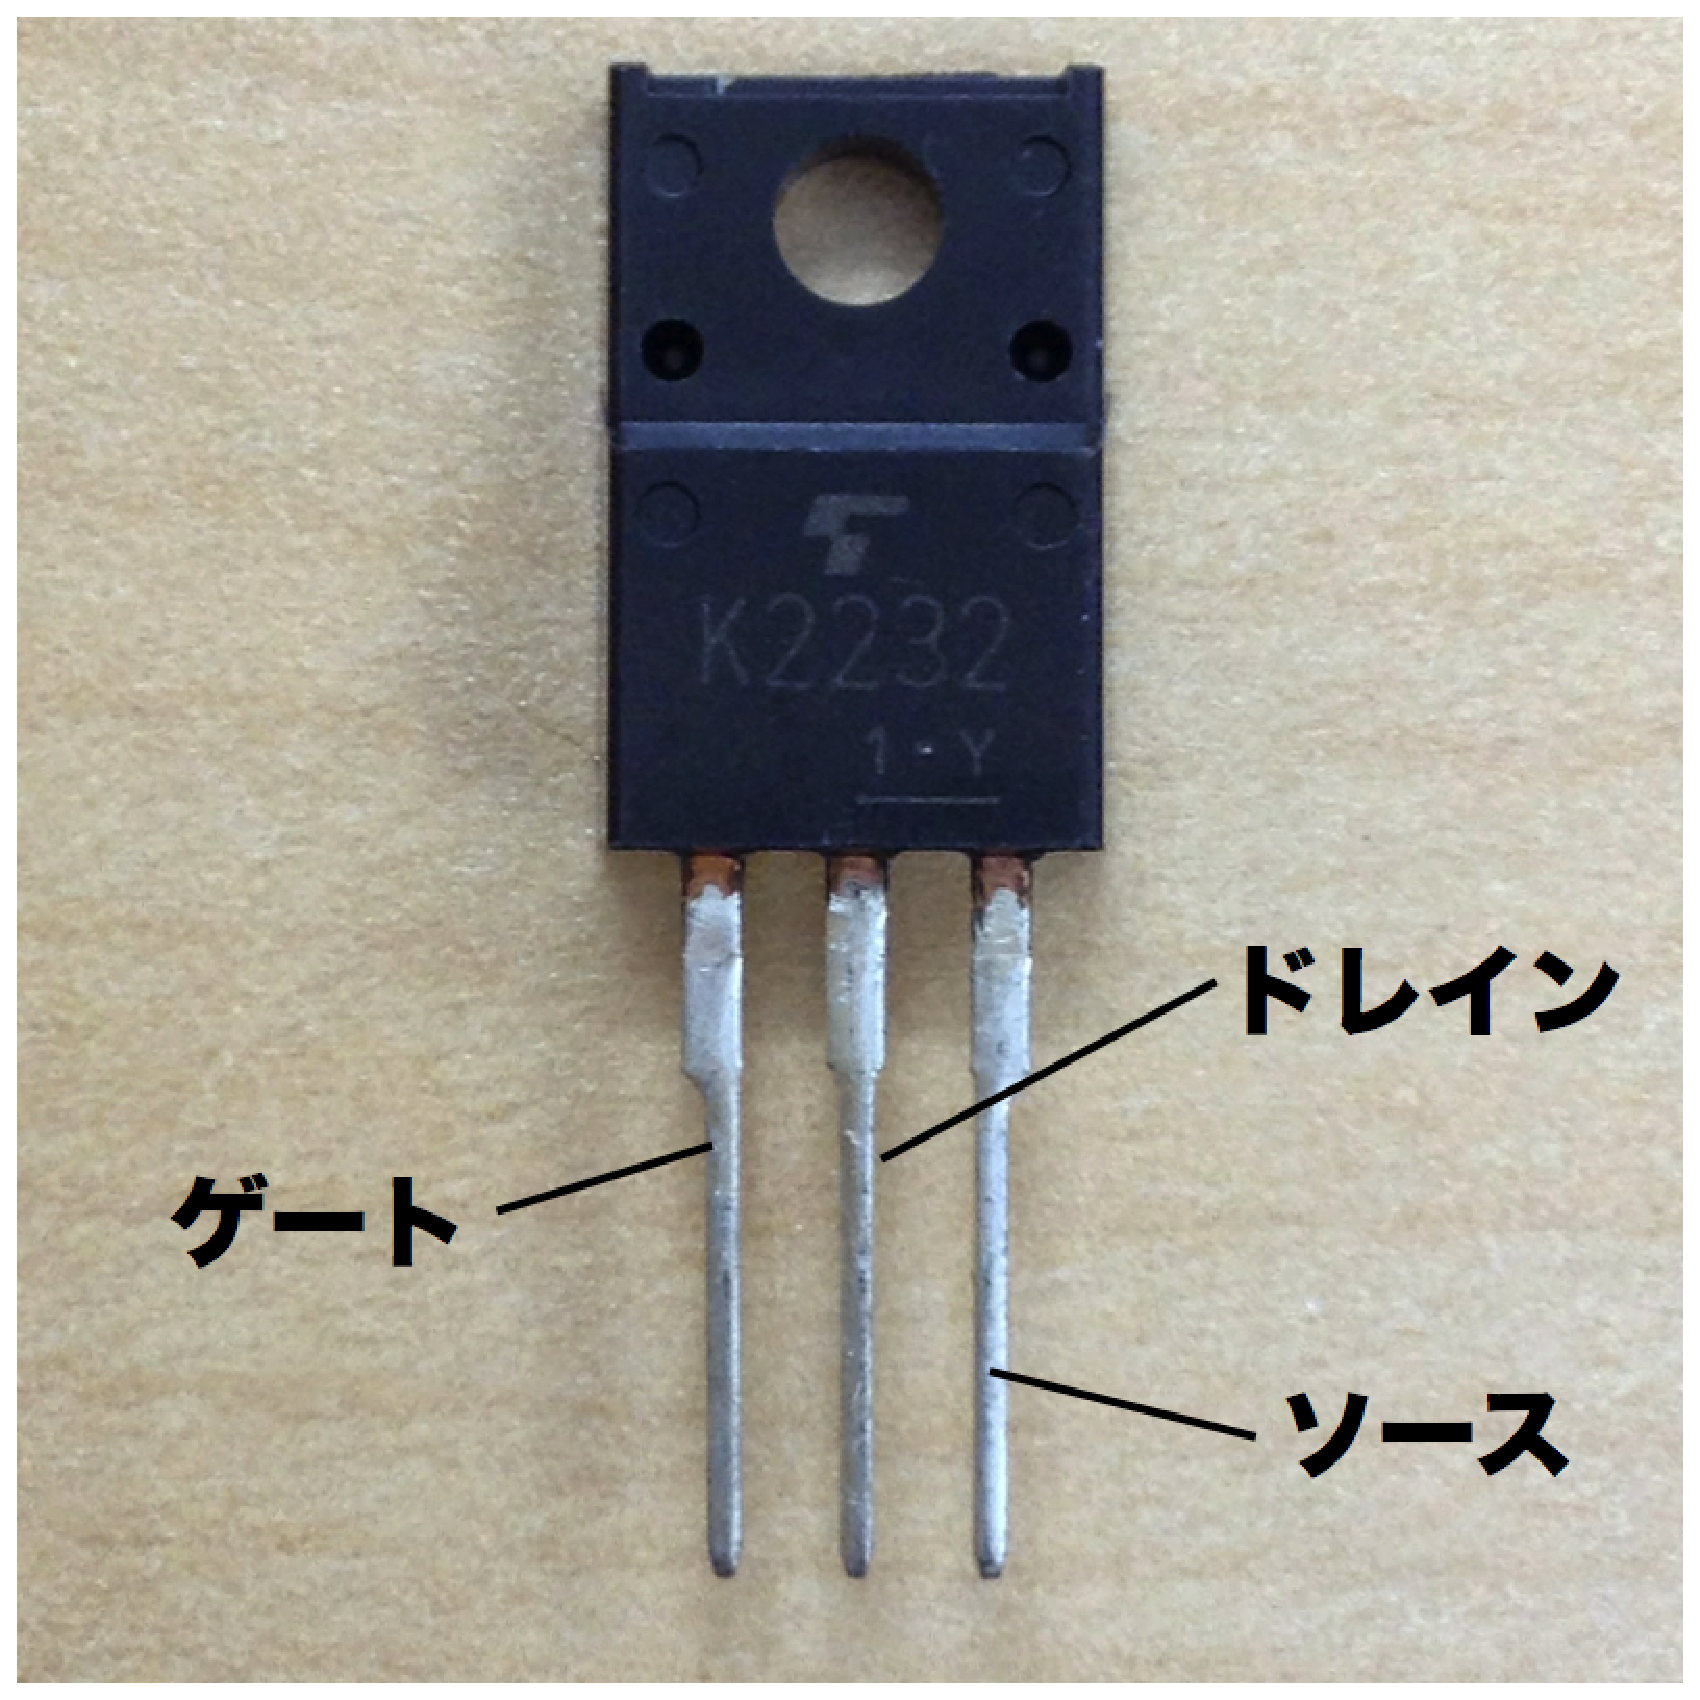
\includegraphics[width=\columnwidth]{img/fet.eps}
  \begin{center}
   \textbf{FET (2SK2232)}
  \end{center}
 \end{minipage}
 \begin{minipage}{0.32\columnwidth}
  \centering
  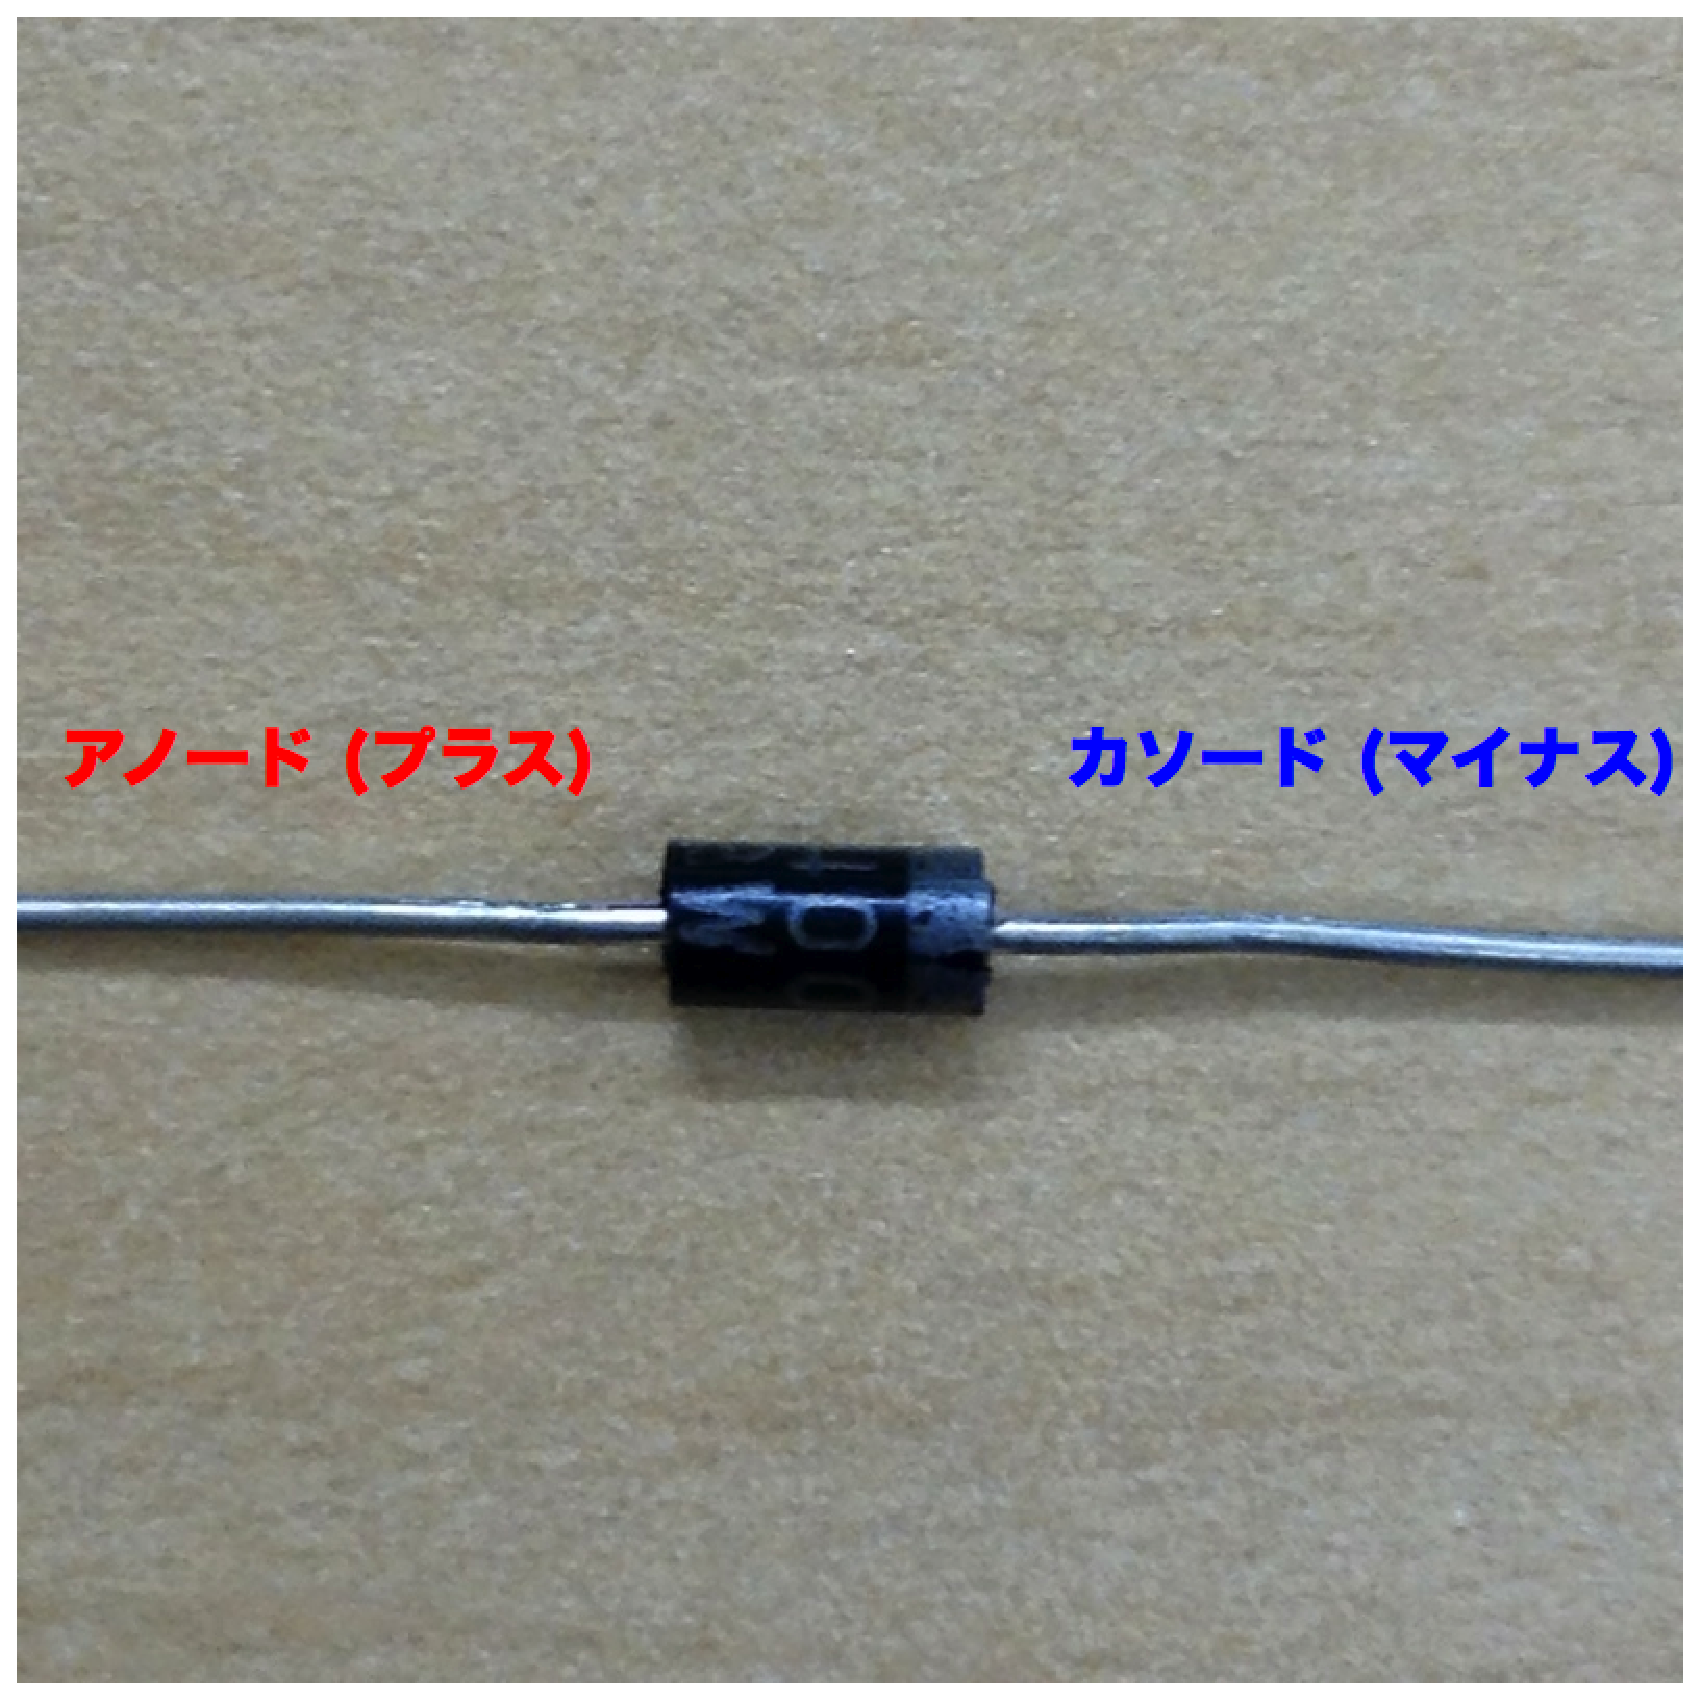
\includegraphics[width=\columnwidth]{img/diode.eps}
  \begin{center}
   \textbf{ダイオード}
  \end{center}
 \end{minipage}
\end{figure}

\subsection*{FETの役割}
FETはゲート・ソース間に電圧を加えることで、ドレイン電流をコントロールできます。図\ref{fet_ID_VGS}に、FETによるゲート・ソース間の電圧とドレイン電流の関係性を示しています。これにより、大きな電流をコントロールしています。

\subsection*{逆起電力}
モーターは電流供給を止めた時などに、慣性でモータが回転してしまうため、モーター自身から逆向きの電流・電圧が流れます。これを逆起電力といいます。この逆起電力によりFETが壊れます。そのため、モーターの両端にダイオードを用いて逆起電力を逃しています。

\begin{figure}[htbp]
 \centering
 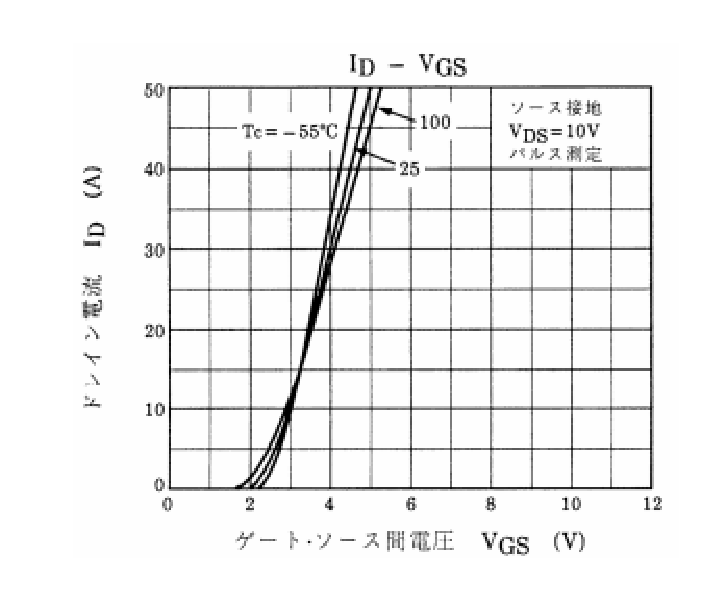
\includegraphics[width=0.5\columnwidth]{img/fet_ID_VGS.eps}
 \begin{center}
  \caption{MOSFETのID--VGS特性}
   \label{fet_ID_VGS}
 \end{center}
\end{figure}

\subsection*{回路}
\begin{figure}[htbp]
 \centering
 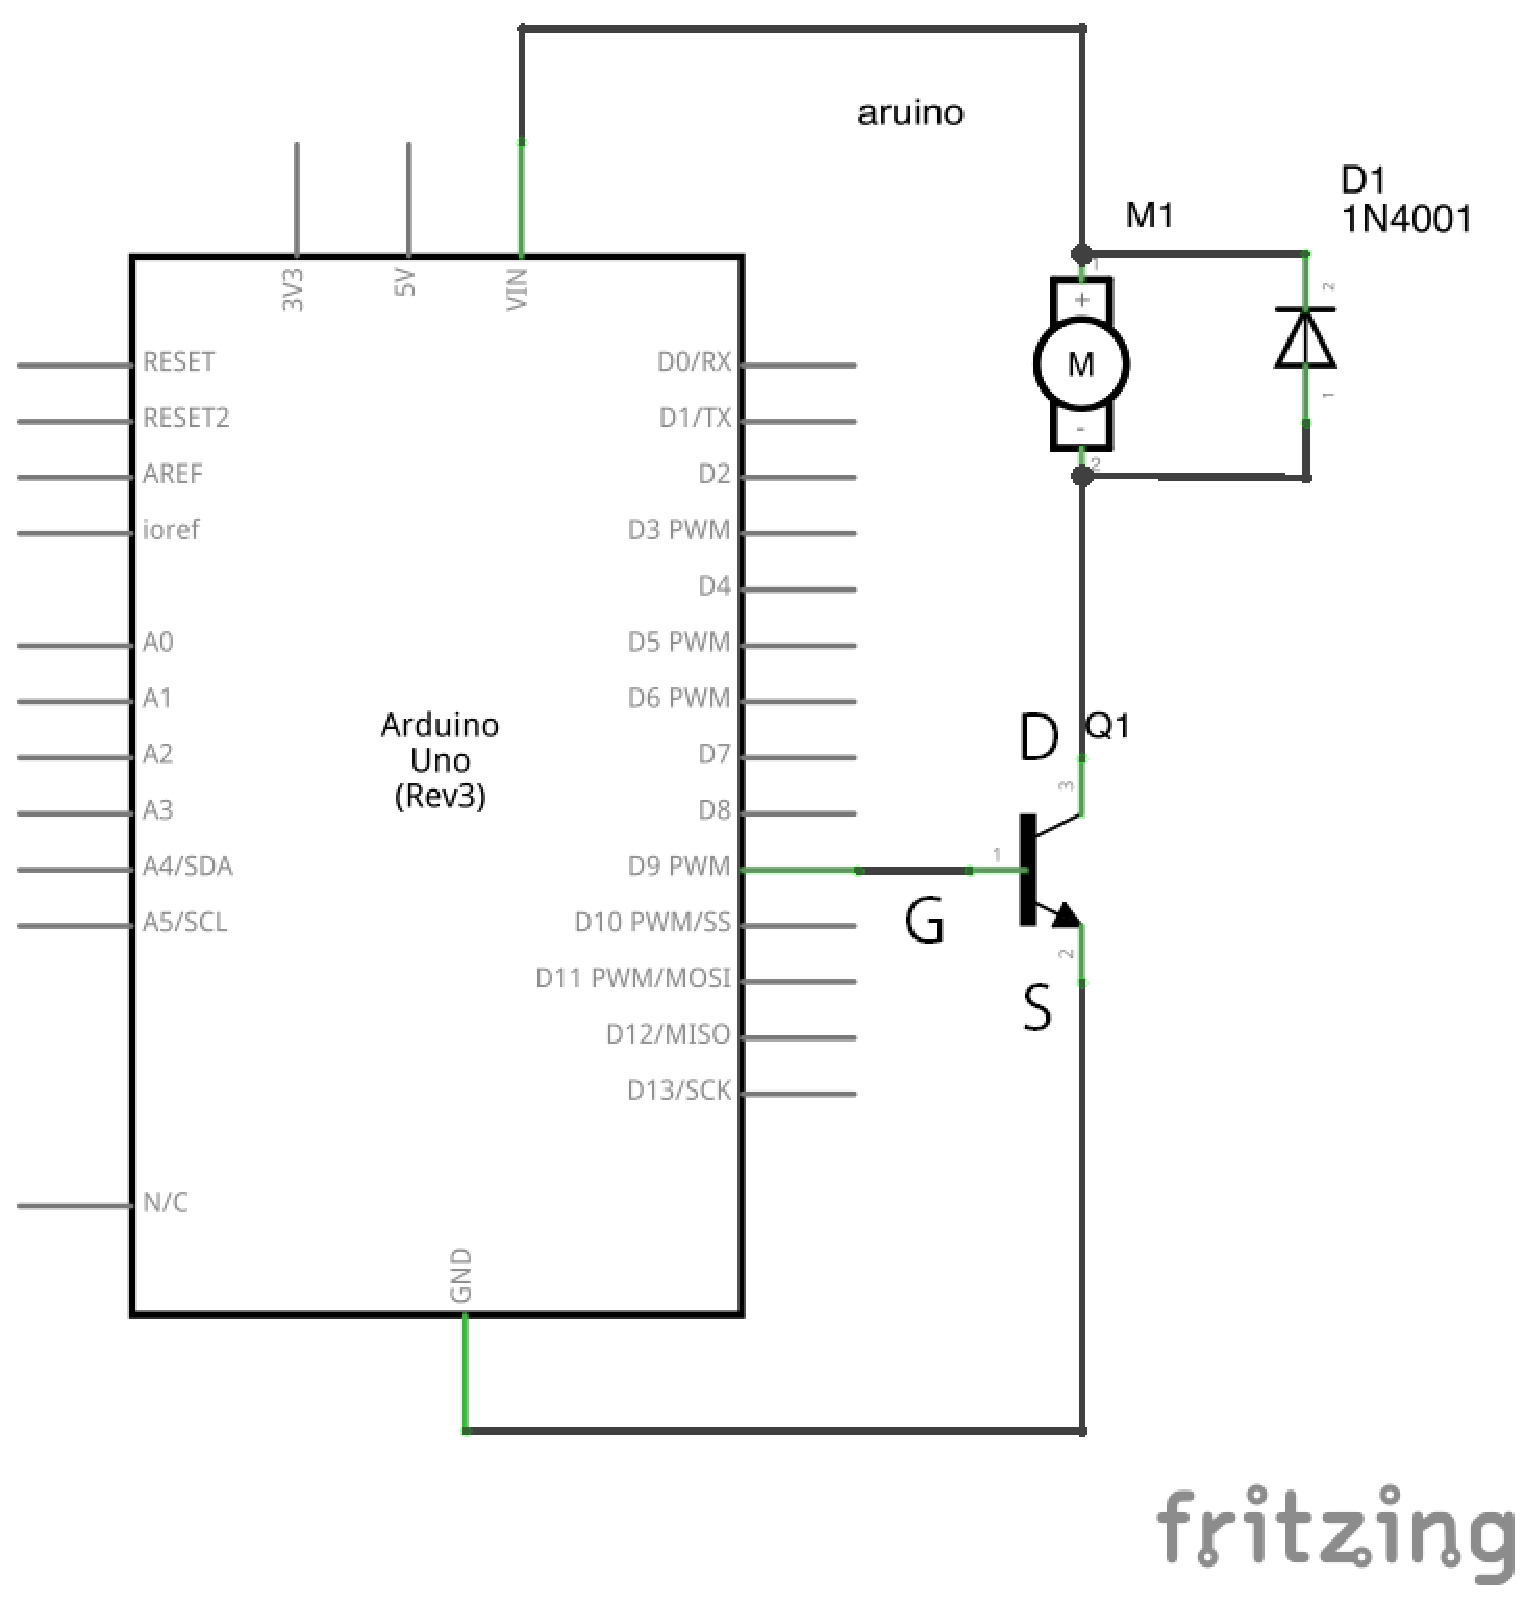
\includegraphics[width=0.5\columnwidth]{img/motor_control_circuit.eps}
 \begin{center}
  \caption{モーター制御のための回路図}
 \end{center}
\end{figure}

\subsection*{プログラム}
\begin{lstlisting}
import processing.serial.*;
import cc.arduino.*;
 
Arduino arduino;
int motorPin = 9;   // モータが接続されたピン
 
void setup() {
  size(255, 255);
  arduino = new Arduino(this, Arduino.list()[5]);
  arduino.pinMode(motorPin, Arduino.OUTPUT);   // モータのピンを出力に設定
}
 
void draw() {
  arduino.analogWrite(motorPin, mouseX);   // モータの回転数をセット
}
\end{lstlisting}


\section{赤外線センサからの入力に基づいてモーターを制御する}
今回の内容を踏まえて、
赤外線センサを用いて取得した距離に基づいて、モーターの回転速度を制御してみよう。
\end{document}